\documentclass[12pt,fleqn]{article}\usepackage{../common}
\begin{document}
Tam Diferansiyel

Bir $f$ fonksiyonunun tam diferansiyeli (total differential) o
fonksiyonun lineerlestirilmesi anlamina gelir. Iki degiskenli bir
fonksiyon icin soyle temsil edilir:

\[ df = f_x(x_0, y_0)dx + f_y(x_0,y_0)dy  \]

Bu formu nasil turetiriz? Bize lazim olan lineerlestirme formulasyonu. Tek
degiskenli bir fonksiyonu lineerlestirmenin teknigi sudur:

\[ L(x) = f(x_0) + f'(x_0) \Delta x  \]

Burada $L(x)$ gercek fonksiyonu yaklasiksal (approximate) olarak temsil eden
lineer fonksiyondur. 

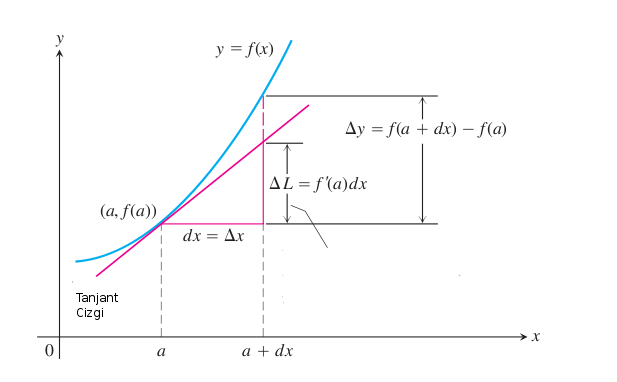
\includegraphics[height=6cm]{linearization.png}

Bu fonksiyonu genisleterek iki degiskenli hale getirelim (sadece $y$
ekleyecegiz)

\[ L(x,y) = f(x_0,y) + f_x(x_0,y) \Delta x \]

Bu fonksiyon da bir onceki kadar ``gecerli''. Sonucta fonksiyonlar
noktasal degerlere gore sonuc verirler, bu sebeple bir lineerlestirme
islemi 2 boyutlu ortamda herhangi bir $x$ noktasinda yapilabildigi
gibi, herhangi bir $x$, $y$ noktasinda da yapilabilir.

Simdi ustteki denklemin sag tarafinda yer alan $f(x_0,y)$'yi lineerlestirelim.  

\[ L(x,y) = L(x_0,y_0) + f_y(x_0,y_0) \Delta y + f_x(x_0,y_0) \Delta x \]

Artik $L(x_0,y_0)$'yi sol tarafa tasiyabiliriz:

\[ \Delta L = L(x,y) - L(x_0,y_0) = f_y(x_0,y_0) \Delta y + f_x(x_0,y_0) \Delta x \]

$\Delta L$ yani $df$ istedigimiz tam diferensiyel sonucudur, $\Delta
x$ yerine $dx$, $\Delta y$ yerine $dy$ kullanabiliriz, o zaman bastaki
formun aynisini elde etmis oluruz.

Turetirken kullandigimiz numarayi uc, dort, vs. gibi istedigimiz kadar
degisken tasiyan $f$ fonksiyonlari icin yapabilirdik, ve sonuc ustteki
forma benzer olurdu. Her degiskenin kismi turevi o degiskenin sonsuz
ufakliktaki ``degisimi'' ile carpilip, o carpimlar toplaninca elimize
tam diferansiyel geciyor.

Kaynaklar

Thomas Calculus 11. Baski

\end{document}